\documentclass[a4paper,12pt,fleqn]{article}
\usepackage{fixltx2e}
\usepackage{helvet}
\usepackage[utf8]{inputenc}
\usepackage{graphicx}
\usepackage{sidecap}
\usepackage{fancyhdr}
\usepackage{amssymb,amsmath}
\usepackage[swedish]{babel}
\usepackage[margin=1.5in]{geometry}
\usepackage{abstract}
\usepackage[parfill]{parskip}
\usepackage{tocloft}
\usepackage{adjustbox}
\usepackage{textcomp}
\usepackage[T1]{fontenc}
\usepackage{listings}
\usepackage{xcolor,colortbl}
\usepackage{hyperref}
\usepackage{mcode}
\usepackage{a4wide}
\usepackage{caption}
\usepackage{helvet}
\usepackage{tocloft}

% Allow footnotes listing so I don't need to quote other sources
\newcommand{\listfootnotesname}{Referenser}% 'List of Footnotes' title 
\newlistof[chapter]{footnotes}{fnt}{\listfootnotesname}% New 'List of...' for footnotes 
\let\oldfootnote\footnote % Save the old \footnote{...} command 
 \renewcommand\footnote[1]{% Redefine the new footnote to also add 'List of Footnote' entries. 
     \refstepcounter{footnotes}% Add and step a reference to the footnote/counter. 
     \oldfootnote{#1}% Make a regular footnote. 
     \addcontentsline{fnt}{footnotes}{\protect 
 \numberline{\thefootnotes}#1}% Add the 'List of...' entry. 
}

% Set sans serif font to Helvetica
%\setsansfont{Helvetica}
% Set serifed font to Cambria
% \setmainfont{Cambria}

\begin{document}

% Titelsida -----------------------------
\begin{titlepage}
\begin{center}

% Upper part of the page. The '~' is needed because \\
% only works if a paragraph has started.

~\\
~\\
\textsc{\LARGE Link{\"o}pings Universitet}\\[1.5cm]


% Title
~\\
~\\
{ \huge \bfseries Teknikhistoria \\ En redogörelse \\[0.4cm] }

% Author and supervisor
\large
\emph{Av:}\\
Hans-Filip \textsc{Elo}

\vfill

% Bottom of the page
{\large \today}

\end{center}

% Slut på titelsida. ---------------------

% ------ Förord
\newpage

\section*{Förord}

I uppgiftsbeskrivningen för denna hemuppgift anges krav på typsättning och grafisk presentation\footnote{Dick Magnusson, Kursanvisningar (TGTU49 HT 14), lisam.liu.se, hämtad 2014-11-17}. Jag har valt att förbise dessa krav då jag ej finner att dessa är representativa för hur jag vill presentera mitt innehåll. Jag har valt att fokusera på läsbarhet och innehåll istället för att låsa mig själv till dessa ramar. Jag hoppas att läsaren finner att läsbarheten är hög och att dispositionen tilltalar denne. 
~\\

Hans-Filip Elo

% Innehåll ------------------------------
\newpage
\thispagestyle{empty}
\tableofcontents
~\\

\begin{center}
\line(1,0){400}
\end{center}

\listoffigures
~\\

\begin{center}
\line(1,0){400}
\end{center}

\listoftables

\end{titlepage}

%header ---------------------------------
\pagestyle{fancy}

\fancyhead{} % clear all header fields
\fancyhead[L]{Hans-Filip Elo \slshape}
\fancyhead[R]{Teknikhistoria - En redogörelse \slshape}

%slut på header ---------------------------------

\section{Inledning}

Människans första kontakt med redskap var i form av skarpt formade stenar som användes för att skära och spetsa föda. Från denna första kontakt har utvecklingen som vi alla vet minst sagt gått långt. Det faktum att denna uppsats skrivs på en högteknologisk skrivmaskin med inbyggd versionshantering och så kallad molnbaserad lagring gör väl denna text till ett så gott bevis som något. 

Tekniken har börjat komma att betyda väldigt mycket för väldigt många. Till en början var redskap och teknik ett sätt att överleva och effektivisera, men idag kan den vara så mycket mer. Tekniken kan idag vara allt ifrån ett ett hjälpmedel, till ett intresse, till ett hinder. 

För undertecknad betalar tekniken min lön och mitt levebröd och den är en starkt utvecklande faktor för min utbildning. Tekniken kan alltså påverka alla våra liv i de mest konstiga riktningar. 

% ---------- Forntid
\newpage

\section{Forntiden}

Redskapen under forntiden var väldigt enkla. Det viktigaste redskapet tros varit handkilen, alltså en vass sten med rundare bakstycke som kan hållas i handen. Handkilar har hittats vars ålder daterats till 2,5 miljoner år. Till en början var redskapen stenar man fann med passande form. Allt eftersom upptäckte man däremot att vissa stenar är hårdare än andra - varpå de hårdare stenarterna användes för att skala stenar av mjukare stenarter till rätt form. 

\begin{figure}[ht!]
\centering
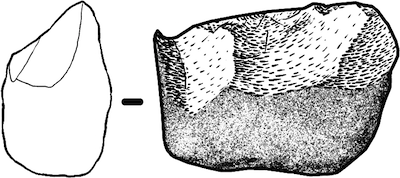
\includegraphics[width=70mm]{handkil.png}
\caption{Skiss av handkil}
\label{handkil}
\end{figure}\footnote{José-Manuel Benito, Creative Commons 3.0 license, \url{http://creativecommons.org/licenses/by-sa/3.0/}}

Handkilen som redskap födde i sin tur andra redskap, framförallt för att tillfångata föda och försvara sig. Med hjälp av handkilen kunde man senare, kring år 40 000 till 10 000 f Kr tillverka mer avancerade redskap såsom kastträ, vassa spjut och harpuner och pilbågar. Från den här tidsperioden har man även funnit grottmålningar.

Forntiden är en väldigt lång tidsperiod, faktiskt större delen av människans existens, men bristen på dokumentation gör att vi får förlita oss på de fynd som görs för att uppskata levnadsförhållanden och teknologisk utveckling. Under senare perioder har människan på eget bevåg dokumenterat mer av sitt leverne, vilket gör att kunskapen om dessa tidsperioder är större. \footnote{Hansson, Staffan. Den skapande människan. 1:a upplagan. Lund: Studentlitteratur, 2002}

\subsection{Människan blir jordbrukare}
I takt med människans utbredning minskade tillgången på större rovdjur, människans primära näringskälla. Bristen på mat ledde till att människan sökte alternativa sätt att finna föda. Den tidiga jordbrukarens redskap bestod framförallt av grävkäppen, en krökt pinne som användes för att underlätta sådd. 

Människan började också senare att ha husdjur. Dessa husdjur innefattade hundar, får, getter, hästar och oxar. I takt med att utvecklingen av fler redskap kom till - så som hackan, skäran och även årdret -  kom höstar och oxar att användas i för att bistå med jordbruket. Genom de nya redskapen och djuren kunde jordbruket öka i skala och bättre försörja en familj. 

Jordbruket gjorde också människan till en mycket mer bofast varelse, vilket möjliggjorde mer permanenta bosättningar. 

\subsection{De första civilisationerna}

I och med den mer bofasta levnadsstilen insåg människan fördelen av att samordna sina boenden. En större grupp är tryggare från attacker av djur och andra människogrupper, och invånarna i en större bosättning kan bistå varandra med olika tjänster. De första större civilisationerna skapades kring ekvatorn, runt några av jordens större floder, kring år 4000 till 3000 f Kr. Att civilisationer skapas först kring ekvatorn och floder är ingen tillfällighet, i o m att tillgången på sötvatten är hög och likaså bördigheten i jorden. 

I och med att bosättningar byggdes i allt större skalor skapade människan ett behov för teknisk utveckling. Man började utveckla byggnads- och bevattningstekniker allt mer för att kunna fylla både mat- och logi till sina civilisationers växande befolkningar. Det är i dessa civilisationer man först funnit bevis på att människan arbetat med brons, alltså en legering mellan tenn och koppar. Bronset hade en betydande del framförallt för vapenproduktion, men till viss del också verktyg. 

De tekniska framstegen inom byggnads och bevattningsteknik gjorde att fler människor kunde få sina levnadsbehov uppfyllda, vilket ledde till att utvecklingen spirade på en rad andra områden. 

I forntidens civilisationer utvecklades det första skriftspråket, i Mesopotamien. Detta skriftspråk, kilskriften, var ett bildligt skriftspråk som använde symboler som beteckning för ord. Egyptens hieroglyfer tros vara influerade av den Mesopotamiska kilskriften. I och med skriftspråket introducerades även tillverkningen av pergament både i Egypten och Mesopotamien. 

% ---------- Antik
\newpage
\section{Antiken}

Efter de forntida civilisationerna startade, kring år 700 f Kr, antiken. Under antiken stod tre civilisationer, Grekland, Kina och Rom som de starkast lysande stjärnorna på den kulturella natthimlen. Grekland ses hos många teoretiker och läror som den västerländska kulturens grundare, och Rom som dess spirituella arvtagare. 

Det största teknologiska arvet från denna period är förmågan att behandla järn till stål. Detta var en tidsödande och tung process där järnet värmdes upp och sedan bankades ut minst 200 gånger. Av denna anledning användes stålet i princip enbart till vapen. Förmågan att tillverka stål är däremot något som är viktigt för framtiden och var en stor del i den industriella revolutionen (ca 1750 till 1870). 

\subsection{Grekland}

Grekland - västvärldens kulturella vagga. Det ses som något ädelt. Antikens Grekland är något som de flesta har goda referenser till. Civilisationen utvecklade i princip alla vetenskapliga områden. Alla former av vetenskap och även jämlikhet (dock mellan män) var saker som prioriterades högt. Grekerna grundlade hela vetenskapliga områden så som matematiken, astrologin, filosofin och fysiken. Strävan efter jämlikhet gjorde också att grekerna skapade världens första försök till en demokratisk stat\footnote{Nationalencyklopedin, http://www.ne.se/uppslagsverk/encyklopedi/l\%C3\%A5ng/demokrati/demokratin-under-antiken, hämtad 2014-11-17}. 

\newpage

I Alexandria, i nuvarande Egypten, i antikens Grekland uppfördes år 300 f Kr världens första universitet, Museion\footnote{Hansson, Staffan. Den skapande människan. 1:a upplagan. Lund: Studentlitteratur, 2002}, där dåtidens forskare och filosofer verkade. Här verkade bland annat Euklides, geometrins fader. En annan känd matematiker från antiken är Pythagoras, mest känd för ''Pythagoras sats'' ($a^2+b^2=c^2$) vilken beskriver förhållandet mellan en rätvinklig triangels sidlängder\footnote{Forsling, Göran, Neymark, Mats. Matematisk analys i en variabel. 2:a upplagan. Linköping: Liber}.

\begin{figure}[ht!]
\centering
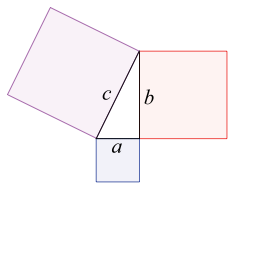
\includegraphics[width=70mm]{pythagoras.png}
\caption{Pythagoras sats}
\label{pythagoras}
\end{figure}\footnote{Michael Hardy, Creative Commons 3.0 license, \url{http://creativecommons.org/licenses/by-sa/3.0/}}

Den mest kända vetenskapsmannen från antikens Grekland får nog ändå ses som filosofen och fysiken Archimedes. Archimedes princip beskriver kroppars förmåga att ''flyta'' respektive ''sjunka'' och är en grundsten inom fysiken. 

Det finns en stor del väldigt kända vetenskapsmän och filosofer från antikens Grekland, men dessa får stå som exempel för den accelererade vetenskapsutvecklingen under den här perioden. Dessa vetenskapliga framsteg får också stå som märke för antikens Grekland i denna text. 

\subsection{Romerska Imperiet}

Romarnas kultur baserade sig till stor del på Greklands, man kopierade exempelvis deras religion och gjorde den till sin egen. Romarriket är det största europeiska riket någonsin. Rent teknologiskt var romarna var pionjärer inom bland annat stridsteknik och -taktik samt vägbyggande. Romarna byggde ett massivt vägnät över det gigantiska riket. Handel via fartyg hade sedan tidigare tagit fart, men i och med romarnas vägbyggande kunde nu befolkningen transportera varor med häst och vagn, om än i mindre utsträckning. 

\subsection{Kinesiska riket}

Kinesiska riket, Mittens rike, var vid den här tiden det teknologiska meckat. Kineserna var i många tekniska tillämpningar århundraden före européerna. Kineserna var framförallt bättre på att gruvverksamhet och metallraffinaderi. Detta i sin tur ledde till många andra teknologiska framsteg som var beroende av järn och stål. 

Kineserna utvann exempelvis salt ur jorden genom att borra med stora stötborrar. Dessa borrar var tillverkade i stål och metallraffineringen var en förutsättning för denna industri. 

Kineserna som också de hade ett stort rike vid den här tiden, hade precis som romarna ett välutvecklat vägnät. Man utvecklade också brobyggande och seldonet. Kinesernas seldon förbättrades. Där tidigare seldon (före 200 f Kr) ströp hästen vid tung last var kinesernas nya seldon mer ergonomiskt. Detta medförde att hästarna kunde dra tyngre släp en längre sträcka. 


% ---------- Medeltiden 
\newpage
\section{Medeltiden}

Medeltiden i Europa inleddes kring år 500 e Kr. 


% ---------- Slutsats
\newpage

\section{Slutsats}

Att den teknologiska utvecklingen gått hand i hand med den sociala, ekonomiska och vetenskapliga utvecklingen är inget att tveka på. Ibland kommer föder den ekonomiska eller sociala utvecklingen ett behov hos tekniken eller vetenskapen, ibland förändrar tekniken eller den vetenskapliga utvecklingen spelfältet för det sociala och ekonomiska landskapet. 

Gemensamt är att teknisk utveckling som sker i öppenhet, eller publika domänen, är det som gett mest mervärde för mänskligheten. En förhoppning från min sida mot framtiden är att allt mer utveckling, framförallt av säkerhetskritiska system, sker i en publik domän. Spionage och brist på öppenhet har förr, framförallt under Kalla Kriget, varit en stor faktor till spänningar inom världspolitiken. Bristen på öppenhet och det allt mer utbredda cyberspionaget kan vara det största framtida teknologiska hotet mot mänskligheten. 

% --------- Källor

\newpage
\addcontentsline{toc}{section}{Referenser}

\listoffootnotes

\end{document}




